\documentclass{standalone}
\usepackage{tikz}
\usetikzlibrary{patterns, positioning}


\begin{document}
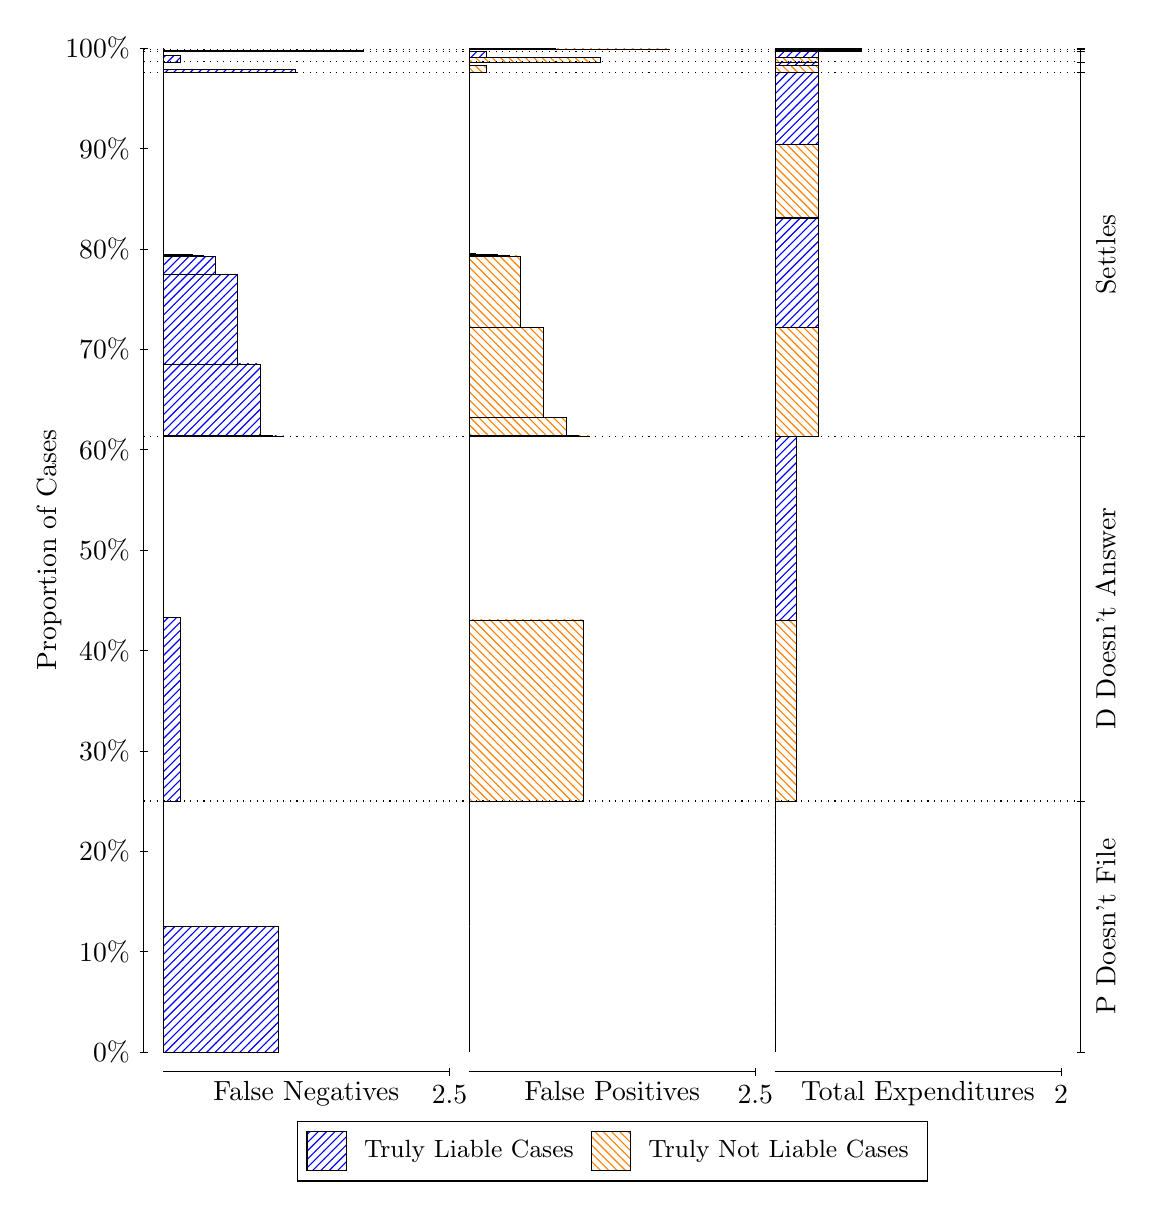
\begin{tikzpicture}
\draw[black, very thin] (1.5,1.75) -- (1.5,14.5);
\node[rotate=90, text=black, anchor=center] at (0.3, 8.125) {Proportion of Cases};
\draw[black, very thin] (1.45,1.75) -- (1.55,1.75);
\node[text=black, anchor=east] at (1.45, 1.75) {0\%};
\draw[black, very thin] (1.45,3.025) -- (1.55,3.025);
\node[text=black, anchor=east] at (1.45, 3.025) {10\%};
\draw[black, very thin] (1.45,4.3) -- (1.55,4.3);
\node[text=black, anchor=east] at (1.45, 4.3) {20\%};
\draw[black, very thin] (1.45,5.575) -- (1.55,5.575);
\node[text=black, anchor=east] at (1.45, 5.575) {30\%};
\draw[black, very thin] (1.45,6.85) -- (1.55,6.85);
\node[text=black, anchor=east] at (1.45, 6.85) {40\%};
\draw[black, very thin] (1.45,8.125) -- (1.55,8.125);
\node[text=black, anchor=east] at (1.45, 8.125) {50\%};
\draw[black, very thin] (1.45,9.4) -- (1.55,9.4);
\node[text=black, anchor=east] at (1.45, 9.4) {60\%};
\draw[black, very thin] (1.45,10.675) -- (1.55,10.675);
\node[text=black, anchor=east] at (1.45, 10.675) {70\%};
\draw[black, very thin] (1.45,11.95) -- (1.55,11.95);
\node[text=black, anchor=east] at (1.45, 11.95) {80\%};
\draw[black, very thin] (1.45,13.225) -- (1.55,13.225);
\node[text=black, anchor=east] at (1.45, 13.225) {90\%};
\draw[black, very thin] (1.45,14.5) -- (1.55,14.5);
\node[text=black, anchor=east] at (1.45, 14.5) {100\%};

\draw[black, very thin] (13.4,1.75) -- (13.4,14.5);
\draw[black, very thin] (13.35,1.75) -- (13.45,1.75);
\node[anchor=west] at (13.35, 1.75) {};
\draw[black, very thin] (13.35,4.9375) -- (13.45,4.9375);
\node[anchor=west] at (13.35, 4.9375) {};
\draw[black, very thin] (13.35,9.5707) -- (13.45,9.5707);
\node[anchor=west] at (13.35, 9.5707) {};
\draw[black, very thin] (13.35,14.188) -- (13.45,14.188);
\node[anchor=west] at (13.35, 14.188) {};
\draw[black, very thin] (13.35,14.325) -- (13.45,14.325);
\node[anchor=west] at (13.35, 14.325) {};
\draw[black, very thin] (13.35,14.46) -- (13.45,14.46);
\node[anchor=west] at (13.35, 14.46) {};
\draw[black, very thin] (13.35,14.48) -- (13.45,14.48);
\node[anchor=west] at (13.35, 14.48) {};
\draw[black, very thin] (13.35,14.5) -- (13.45,14.5);
\node[anchor=west] at (13.35, 14.5) {};

\draw[black, very thin, pattern color=blue, pattern=north east lines] (1.75,1.75) rectangle (3.2033,3.3438);
\draw[black, very thin, pattern color=orange, pattern=north west lines] (1.75,3.3438) rectangle (1.75,4.9375);
\draw[black, very thin, pattern color=blue, pattern=north east lines] (1.75,4.9375) rectangle (1.968,7.272);
\draw[black, very thin, pattern color=orange, pattern=north west lines] (1.75,7.272) rectangle (1.75,9.5707);
\draw[black, very thin, pattern color=blue, pattern=north east lines] (1.75,9.5707) rectangle (3.276,9.5739);
\draw[black, very thin, pattern color=blue, pattern=north east lines] (1.75,9.5739) rectangle (3.1307,9.5776);
\draw[black, very thin, pattern color=blue, pattern=north east lines] (1.75,9.5776) rectangle (2.9853,10.489);
\draw[black, very thin, pattern color=blue, pattern=north east lines] (1.75,10.489) rectangle (2.84,10.489);
\draw[black, very thin, pattern color=blue, pattern=north east lines] (1.75,10.489) rectangle (2.6947,11.628);
\draw[black, very thin, pattern color=blue, pattern=north east lines] (1.75,11.628) rectangle (2.5493,11.628);
\draw[black, very thin, pattern color=blue, pattern=north east lines] (1.75,11.628) rectangle (2.404,11.856);
\draw[black, very thin, pattern color=blue, pattern=north east lines] (1.75,11.856) rectangle (2.2587,11.862);
\draw[black, very thin, pattern color=blue, pattern=north east lines] (1.75,11.862) rectangle (2.1133,11.875);
\draw[black, very thin, pattern color=orange, pattern=north west lines] (1.75,11.875) rectangle (1.75,14.188);
\draw[black, very thin, pattern color=blue, pattern=north east lines] (1.75,14.188) rectangle (3.4213,14.233);
\draw[black, very thin, pattern color=orange, pattern=north west lines] (1.75,14.233) rectangle (1.75,14.325);
\draw[black, very thin, pattern color=blue, pattern=north east lines] (1.75,14.325) rectangle (1.968,14.403);
\draw[black, very thin, pattern color=orange, pattern=north west lines] (1.75,14.403) rectangle (1.75,14.46);
\draw[black, very thin, pattern color=blue, pattern=north east lines] (1.75,14.46) rectangle (4.2933,14.467);
\draw[black, very thin, pattern color=orange, pattern=north west lines] (1.75,14.467) rectangle (1.75,14.48);
\draw[black, very thin, pattern color=orange, pattern=north west lines] (1.75,14.48) rectangle (1.75,14.488);
\draw[black, very thin, pattern color=blue, pattern=north east lines] (1.75,14.488) rectangle (1.75,14.5);
\draw[black, very thin, pattern color=orange, pattern=north west lines] (5.6333,1.75) rectangle (5.6333,3.3437);
\draw[black, very thin, pattern color=blue, pattern=north east lines] (5.6333,3.3437) rectangle (5.6333,4.9375);
\draw[black, very thin, pattern color=orange, pattern=north west lines] (5.6333,4.9375) rectangle (7.0867,7.2361);
\draw[black, very thin, pattern color=blue, pattern=north east lines] (5.6333,7.2361) rectangle (5.6333,9.5707);
\draw[black, very thin, pattern color=orange, pattern=north west lines] (5.6333,9.5707) rectangle (7.1593,9.5756);
\draw[black, very thin, pattern color=orange, pattern=north west lines] (5.6333,9.5756) rectangle (7.014,9.5813);
\draw[black, very thin, pattern color=orange, pattern=north west lines] (5.6333,9.5813) rectangle (6.8687,9.8096);
\draw[black, very thin, pattern color=orange, pattern=north west lines] (5.6333,9.8096) rectangle (6.7233,9.8098);
\draw[black, very thin, pattern color=orange, pattern=north west lines] (5.6333,9.8098) rectangle (6.578,10.949);
\draw[black, very thin, pattern color=orange, pattern=north west lines] (5.6333,10.949) rectangle (6.4327,10.95);
\draw[black, very thin, pattern color=orange, pattern=north west lines] (5.6333,10.95) rectangle (6.2873,11.861);
\draw[black, very thin, pattern color=orange, pattern=north west lines] (5.6333,11.861) rectangle (6.142,11.869);
\draw[black, very thin, pattern color=orange, pattern=north west lines] (5.6333,11.869) rectangle (5.9967,11.884);
\draw[black, very thin, pattern color=blue, pattern=north east lines] (5.6333,11.884) rectangle (5.706,11.896);
\draw[black, very thin, pattern color=blue, pattern=north east lines] (5.6333,11.896) rectangle (5.6333,14.188);
\draw[black, very thin, pattern color=orange, pattern=north west lines] (5.6333,14.188) rectangle (5.8513,14.28);
\draw[black, very thin, pattern color=blue, pattern=north east lines] (5.6333,14.28) rectangle (5.6333,14.325);
\draw[black, very thin, pattern color=orange, pattern=north west lines] (5.6333,14.325) rectangle (7.3047,14.382);
\draw[black, very thin, pattern color=blue, pattern=north east lines] (5.6333,14.382) rectangle (5.8513,14.46);
\draw[black, very thin, pattern color=orange, pattern=north west lines] (5.6333,14.46) rectangle (5.6333,14.473);
\draw[black, very thin, pattern color=blue, pattern=north east lines] (5.6333,14.473) rectangle (5.6333,14.48);
\draw[black, very thin, pattern color=orange, pattern=north west lines] (5.6333,14.48) rectangle (8.1767,14.488);
\draw[black, very thin, pattern color=blue, pattern=north east lines] (5.6333,14.488) rectangle (6.7233,14.5);
\draw[black, very thin, pattern color=orange, pattern=north west lines] (9.5167,1.75) rectangle (9.5167,3.3437);
\draw[black, very thin, pattern color=blue, pattern=north east lines] (9.5167,3.3437) rectangle (9.5167,4.9375);
\draw[black, very thin, pattern color=orange, pattern=north west lines] (9.5167,4.9375) rectangle (9.7892,7.2361);
\draw[black, very thin, pattern color=blue, pattern=north east lines] (9.5167,7.2361) rectangle (9.7892,9.5707);
\draw[black, very thin, pattern color=orange, pattern=north west lines] (9.5167,9.5707) rectangle (10.062,10.949);
\draw[black, very thin, pattern color=blue, pattern=north east lines] (9.5167,10.949) rectangle (10.062,12.336);
\draw[black, very thin, pattern color=orange, pattern=north west lines] (9.5167,12.336) rectangle (10.062,12.35);
\draw[black, very thin, pattern color=blue, pattern=north east lines] (9.5167,12.35) rectangle (10.062,12.353);
\draw[black, very thin, pattern color=orange, pattern=north west lines] (9.5167,12.353) rectangle (10.062,13.273);
\draw[black, very thin, pattern color=blue, pattern=north east lines] (9.5167,13.273) rectangle (10.062,14.188);
\draw[black, very thin, pattern color=orange, pattern=north west lines] (9.5167,14.188) rectangle (10.062,14.28);
\draw[black, very thin, pattern color=blue, pattern=north east lines] (9.5167,14.28) rectangle (10.062,14.325);
\draw[black, very thin, pattern color=orange, pattern=north west lines] (9.5167,14.325) rectangle (10.062,14.382);
\draw[black, very thin, pattern color=blue, pattern=north east lines] (9.5167,14.382) rectangle (10.062,14.46);
\draw[black, very thin, pattern color=orange, pattern=north west lines] (9.5167,14.46) rectangle (10.607,14.473);
\draw[black, very thin, pattern color=blue, pattern=north east lines] (9.5167,14.473) rectangle (10.607,14.48);
\draw[black, very thin, pattern color=orange, pattern=north west lines] (9.5167,14.48) rectangle (10.607,14.488);
\draw[black, very thin, pattern color=blue, pattern=north east lines] (9.5167,14.488) rectangle (10.607,14.5);
\draw[black, dotted] (1.5,4.9375) -- (13.4,4.9375);
\draw[black, dotted] (1.5,9.5707) -- (13.4,9.5707);
\draw[black, dotted] (1.5,14.188) -- (13.4,14.188);
\draw[black, dotted] (1.5,14.325) -- (13.4,14.325);
\draw[black, dotted] (1.5,14.46) -- (13.4,14.46);
\draw[black, dotted] (1.5,14.48) -- (13.4,14.48);
\draw[black, very thin] (1.75,1.5) -- (5.3833,1.5);
\node[text=black, anchor=north] at (3.5667, 1.5) {False Negatives};
\draw[black, very thin] (5.3833,1.45) -- (5.3833,1.55);
\node[text=black, anchor=north] at (5.3833, 1.45) {2.5};

\draw[black, very thin] (5.6333,1.5) -- (9.2667,1.5);
\node[text=black, anchor=north] at (7.45, 1.5) {False Positives};
\draw[black, very thin] (9.2667,1.45) -- (9.2667,1.55);
\node[text=black, anchor=north] at (9.2667, 1.45) {2.5};

\draw[black, very thin] (9.5167,1.5) -- (13.15,1.5);
\node[text=black, anchor=north] at (11.333, 1.5) {Total Expenditures};
\draw[black, very thin] (13.15,1.45) -- (13.15,1.55);
\node[text=black, anchor=north] at (13.15, 1.45) {2};

\node[text=black, centered, rotate=90] at (13.72, 3.3437) {P Doesn't File};
\node[text=black, centered, rotate=90] at (13.72, 7.2541) {D Doesn't Answer};
\node[text=black, centered, rotate=90] at (13.72, 11.879) {Settles};





\draw (7.449999999999999,1.5) node[draw=none] (baseCoordinate) {};
\begin{scope}[align=center]
        \matrix[scale=0.5, draw=black, below=0.5cm of baseCoordinate, nodes={draw}, column sep=0.1cm]{
            \node[rectangle, draw, minimum width=0.5cm, minimum height=0.5cm, pattern color=blue, pattern=north east lines] {}; &
            \node[draw=none, font=\small, text=black] (B) {Truly Liable Cases}; &
            \node[rectangle, draw, minimum width=0.5cm, minimum height=0.5cm, pattern color=orange, pattern=north west lines] {}; &
            \node[draw=none, font=\small, text=black] (B) {Truly Not Liable Cases}; \\
            };
\end{scope}

\end{tikzpicture}
\end{document}